% Show important proofs
% show the foundational sätze they use
\begin{frame}{Example: Only Linear Terms}
  \begin{columns}
    \column{0.5\textwidth}
      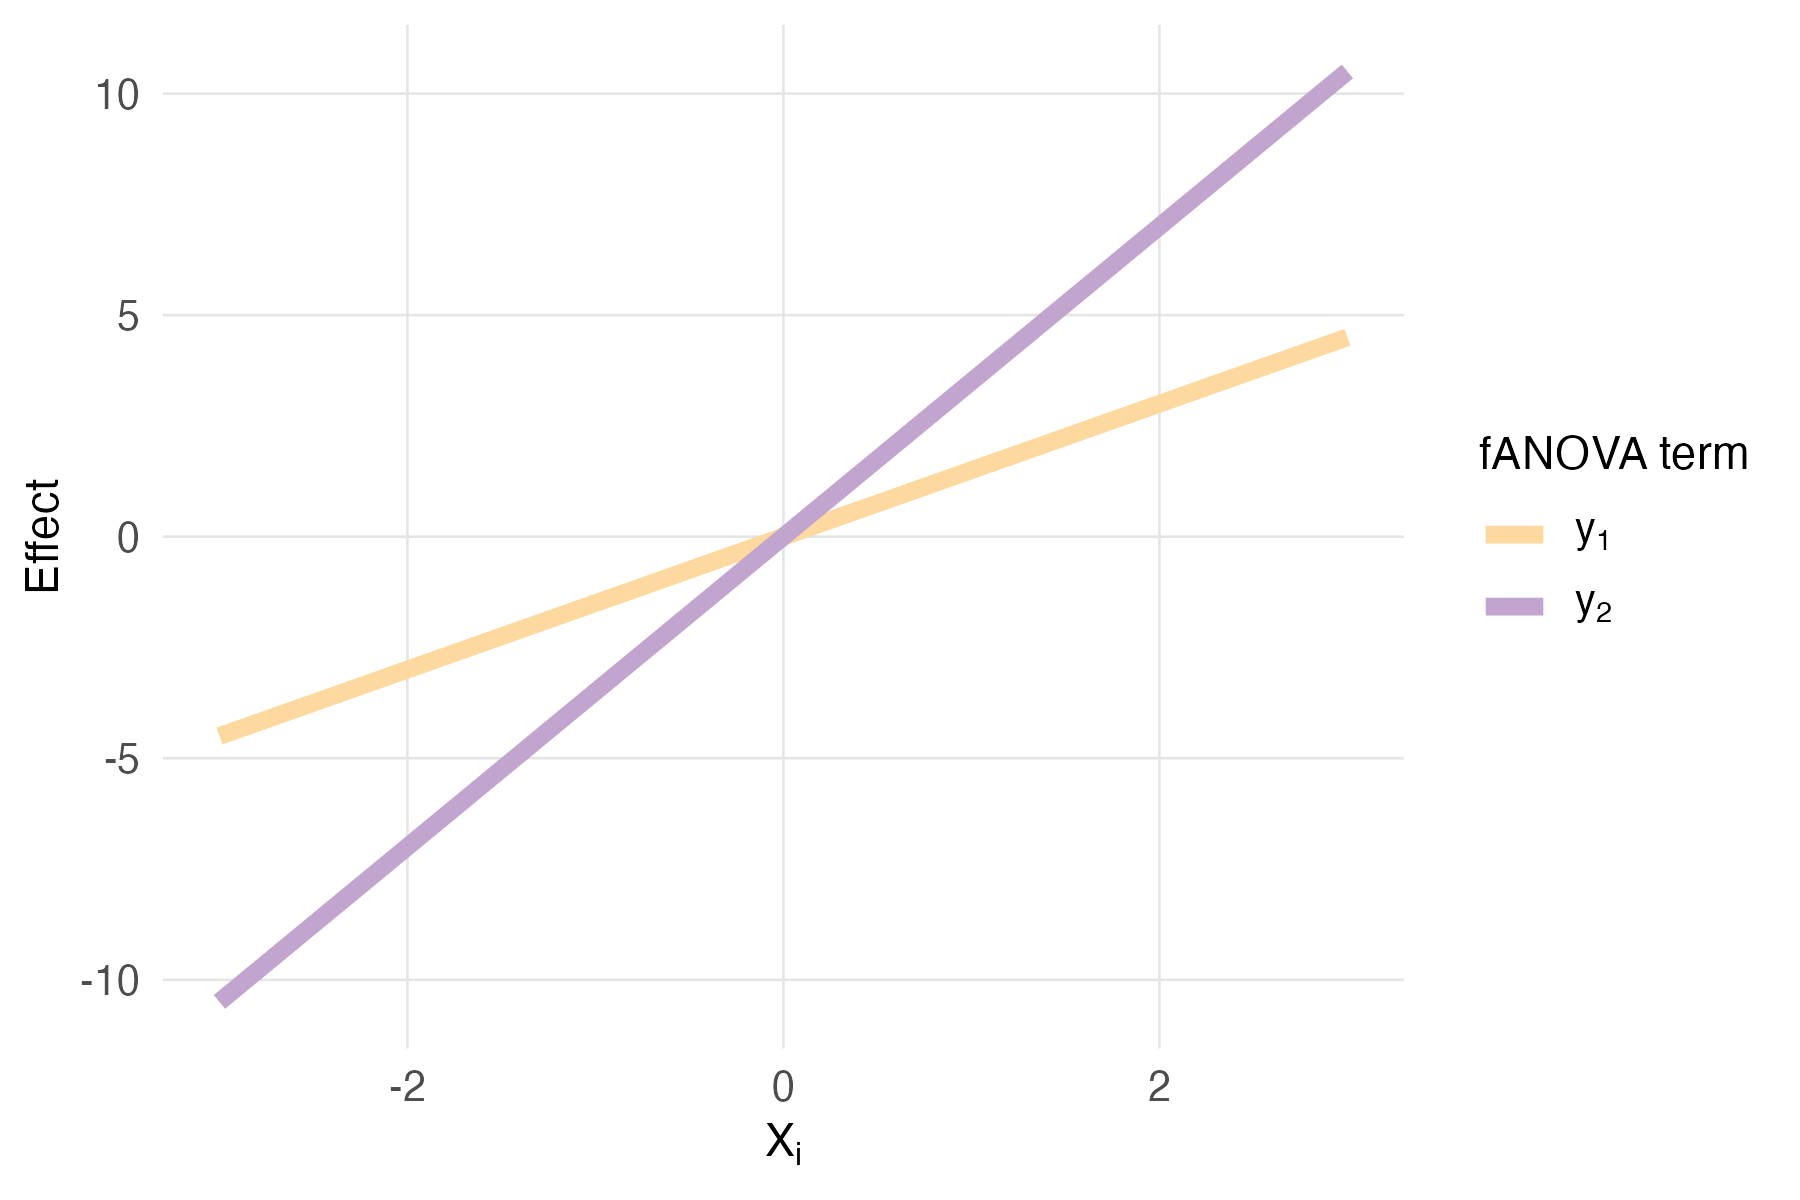
\includegraphics[width=\linewidth]{../images/experiment_section/linear_a1p15_a2p35_a11p00_a22p00_a12p00_rhop00_main.png}
      \captionof{figure}{$q(x_1, x_2) = 1.5 x_1 + 3.5 x_2$}
    \column{0.5\textwidth}
      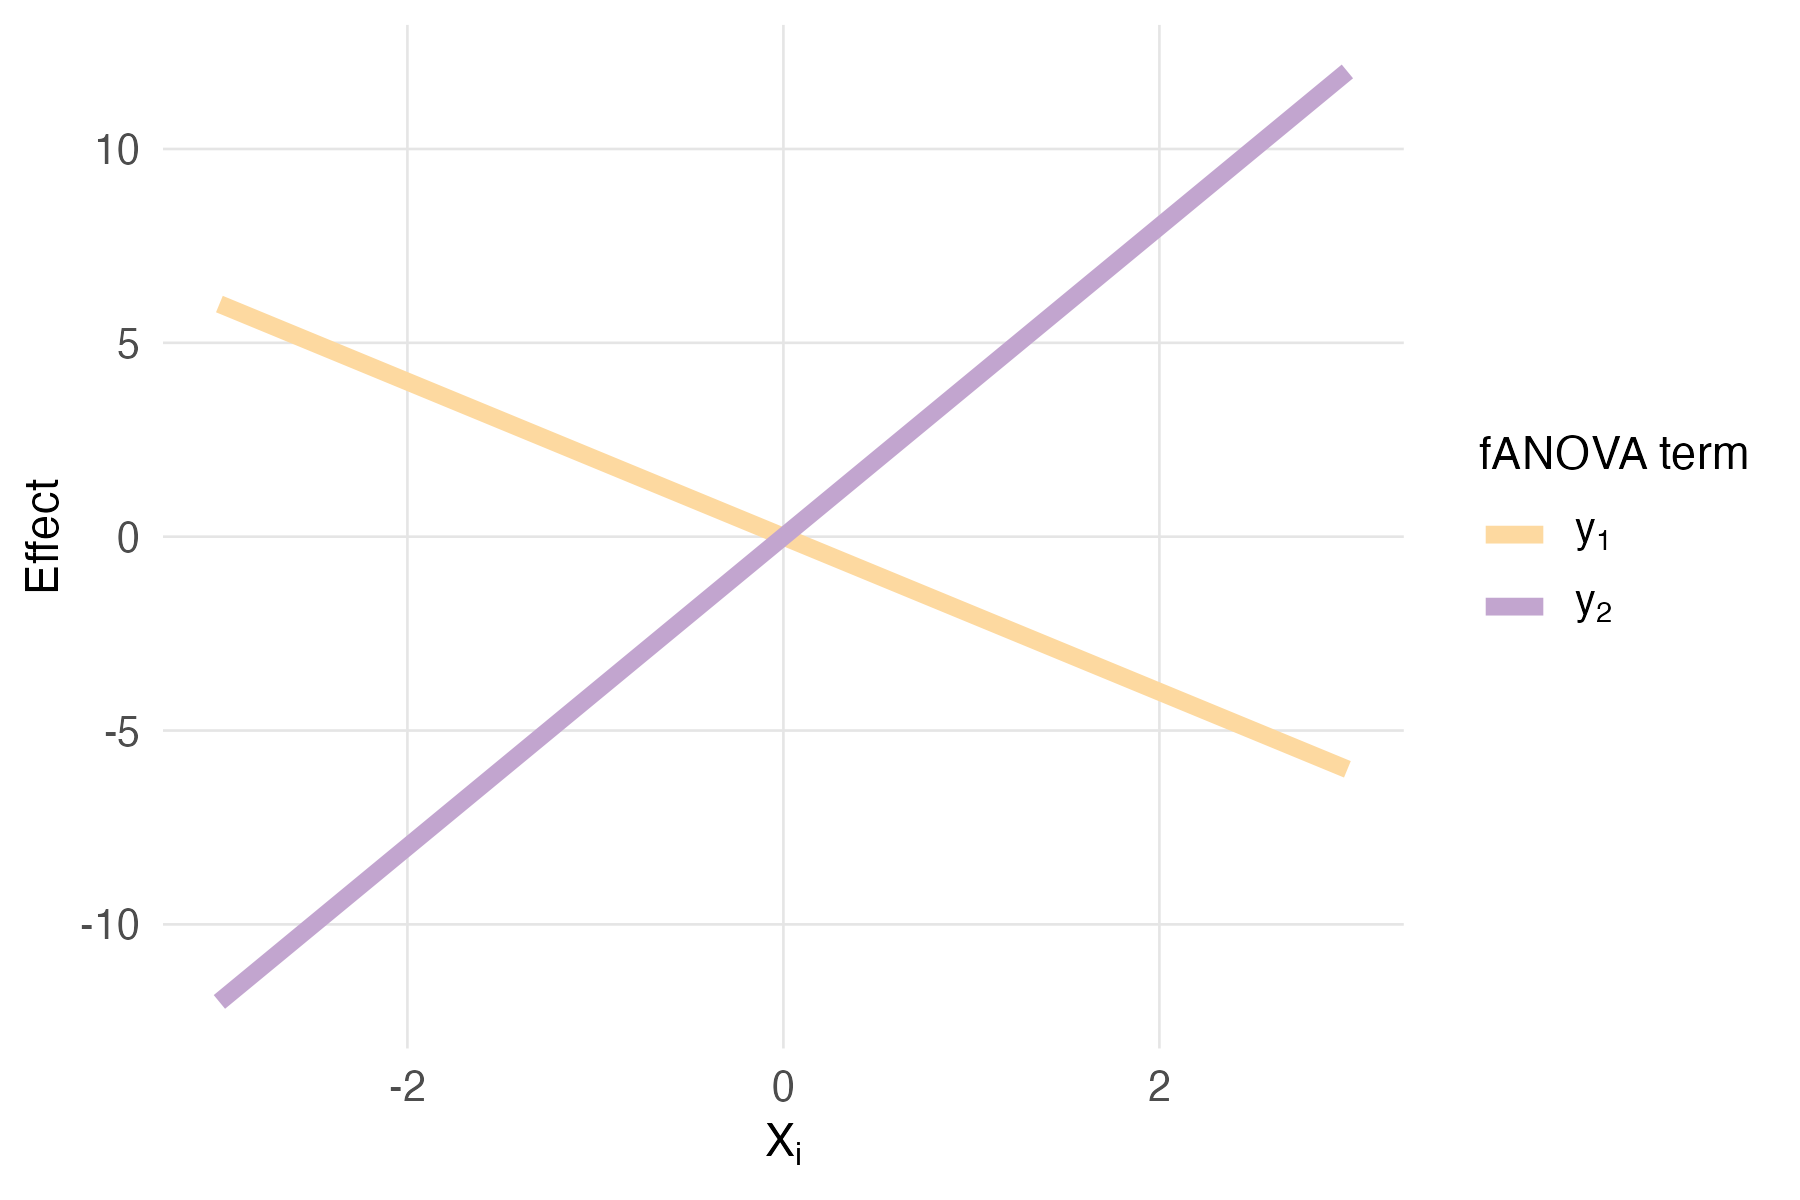
\includegraphics[width=\linewidth]{../images/experiment_section/linear_a1m20_a2p40_a11p00_a22p00_a12p00_rhop00_main.png}
      \captionof{figure}{$q(x_1, x_2) = -2 x_1 + 4 x_2$}
  \end{columns}
\end{frame}

\begin{frame}{Example: Interaction}
  \[
  y(x_1, x_2) = x_1 x_2 \qquad \rho = -0.5
  \]
    \begin{columns}
    \column{0.5\textwidth}
      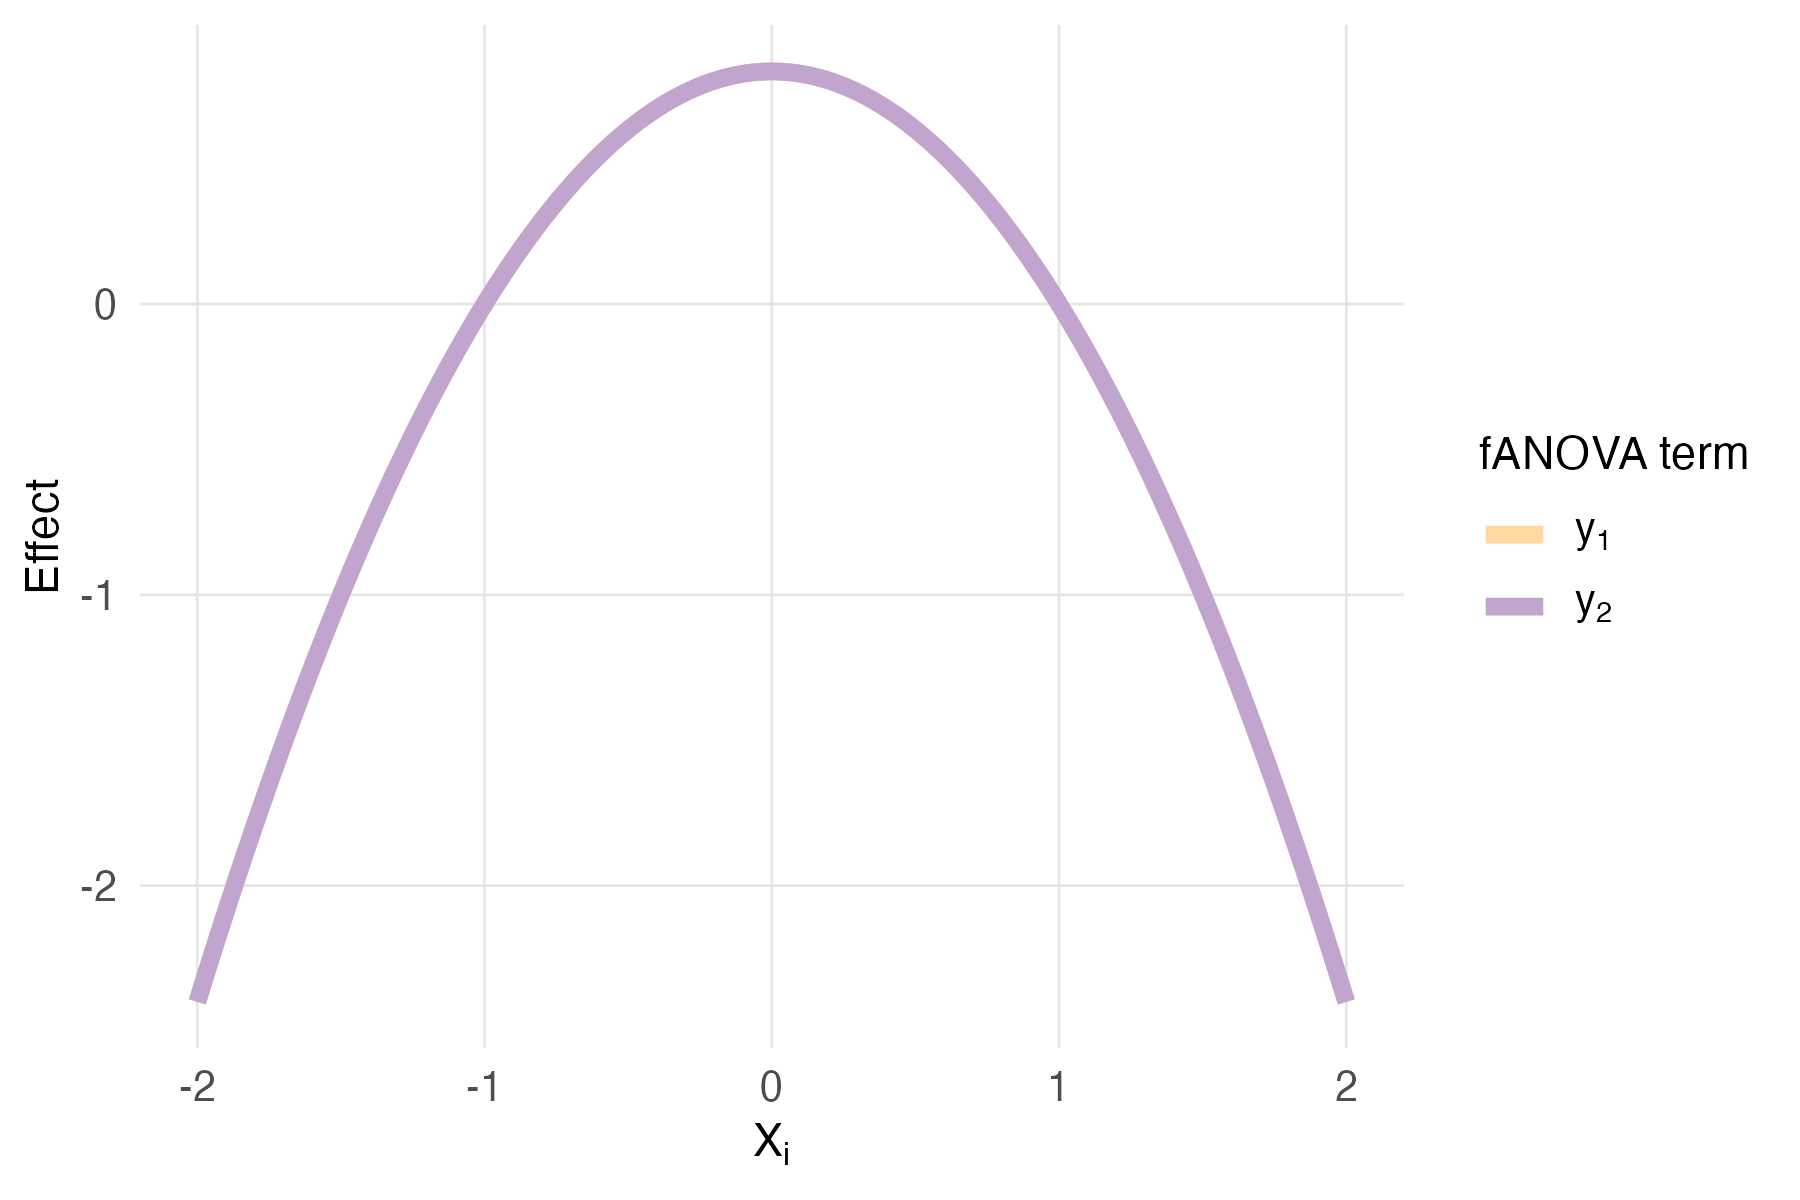
\includegraphics[width=\linewidth]{../images/experiment_section/interaction_a1p00_a2p00_a11p00_a22p00_a12p20_rhom05_main.png}
    \column{0.5\textwidth}
      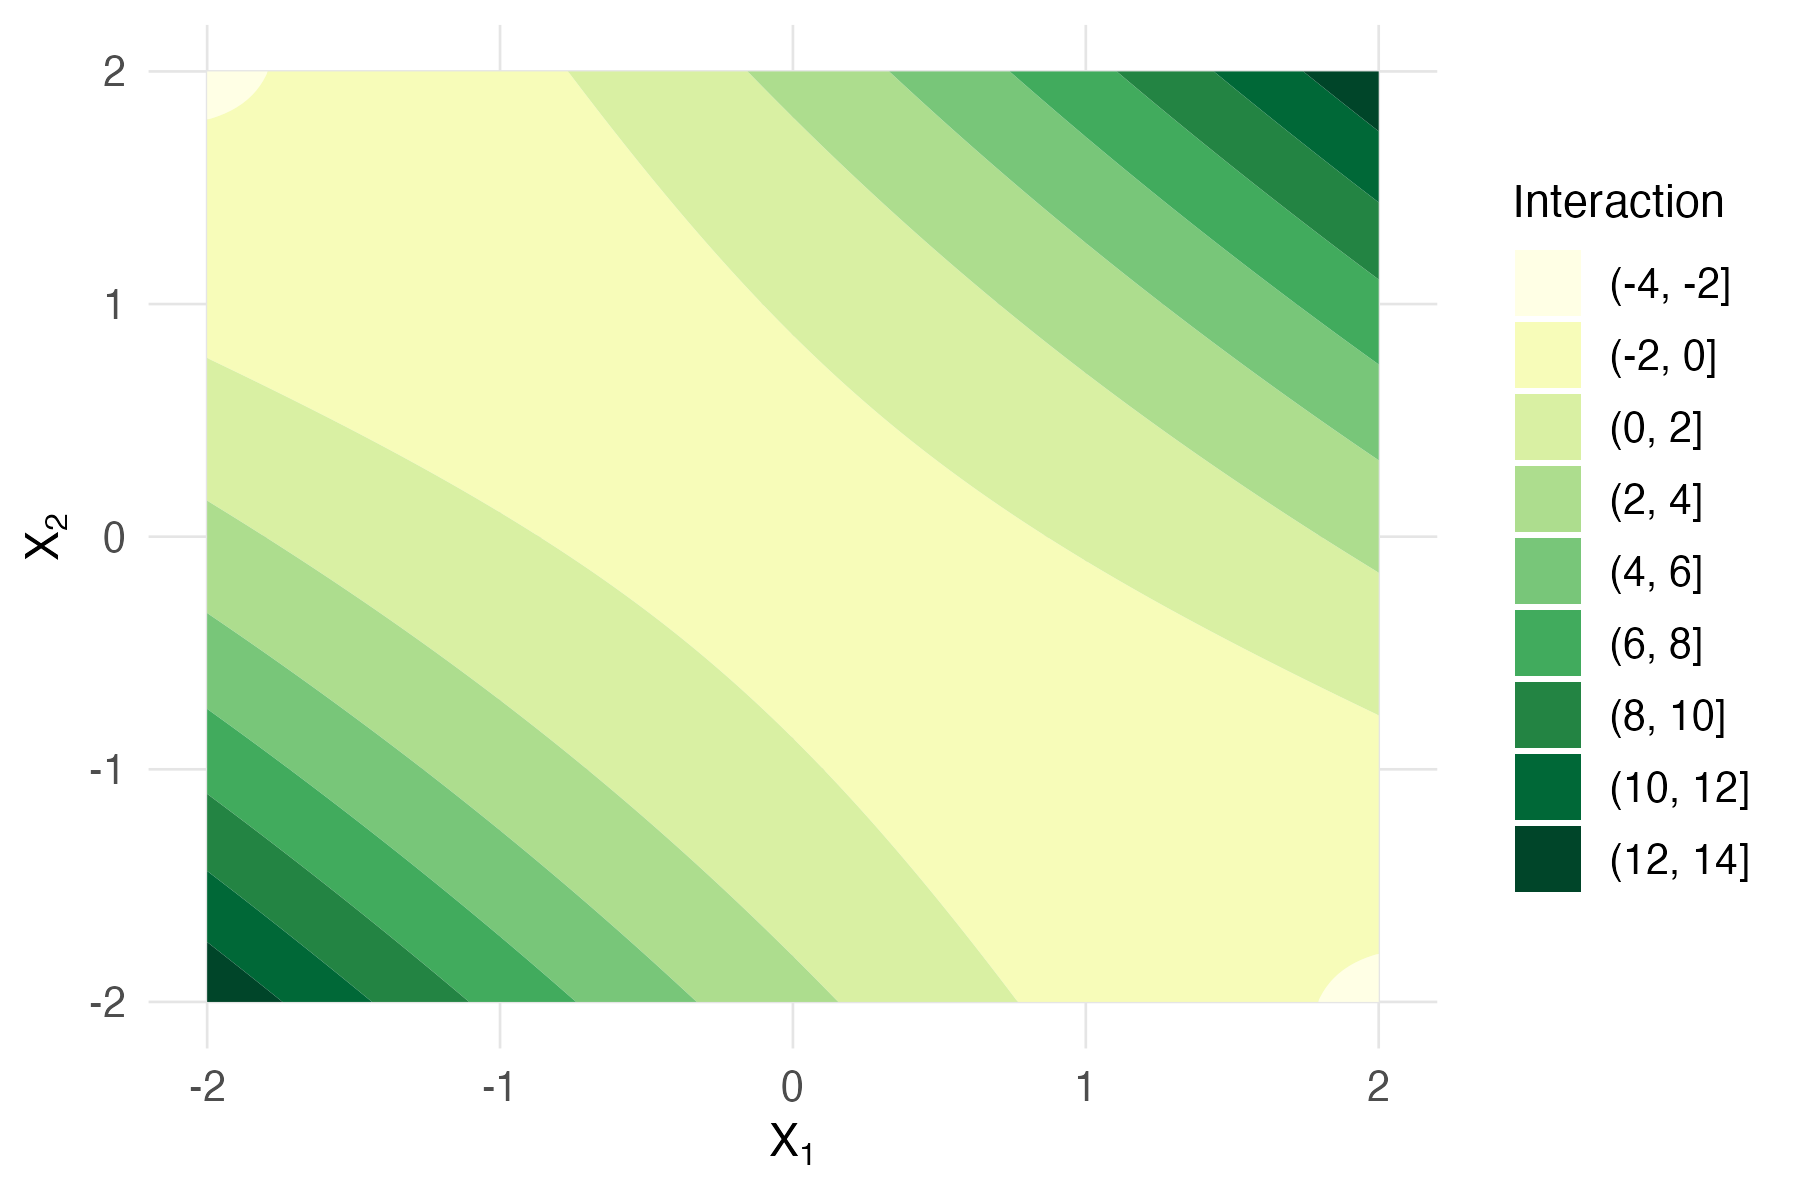
\includegraphics[width=\linewidth]{../images/experiment_section/interaction_a1p00_a2p00_a11p00_a22p00_a12p20_rhom05_interaction.png}
  \end{columns}
  
\end{frame}

\begin{frame}{Example: Interaction}
  \[
  y(x_1, x_2) = x_1 x_2 \qquad \rho = 0
  \]
    \begin{columns}
    \column{0.5\textwidth}
      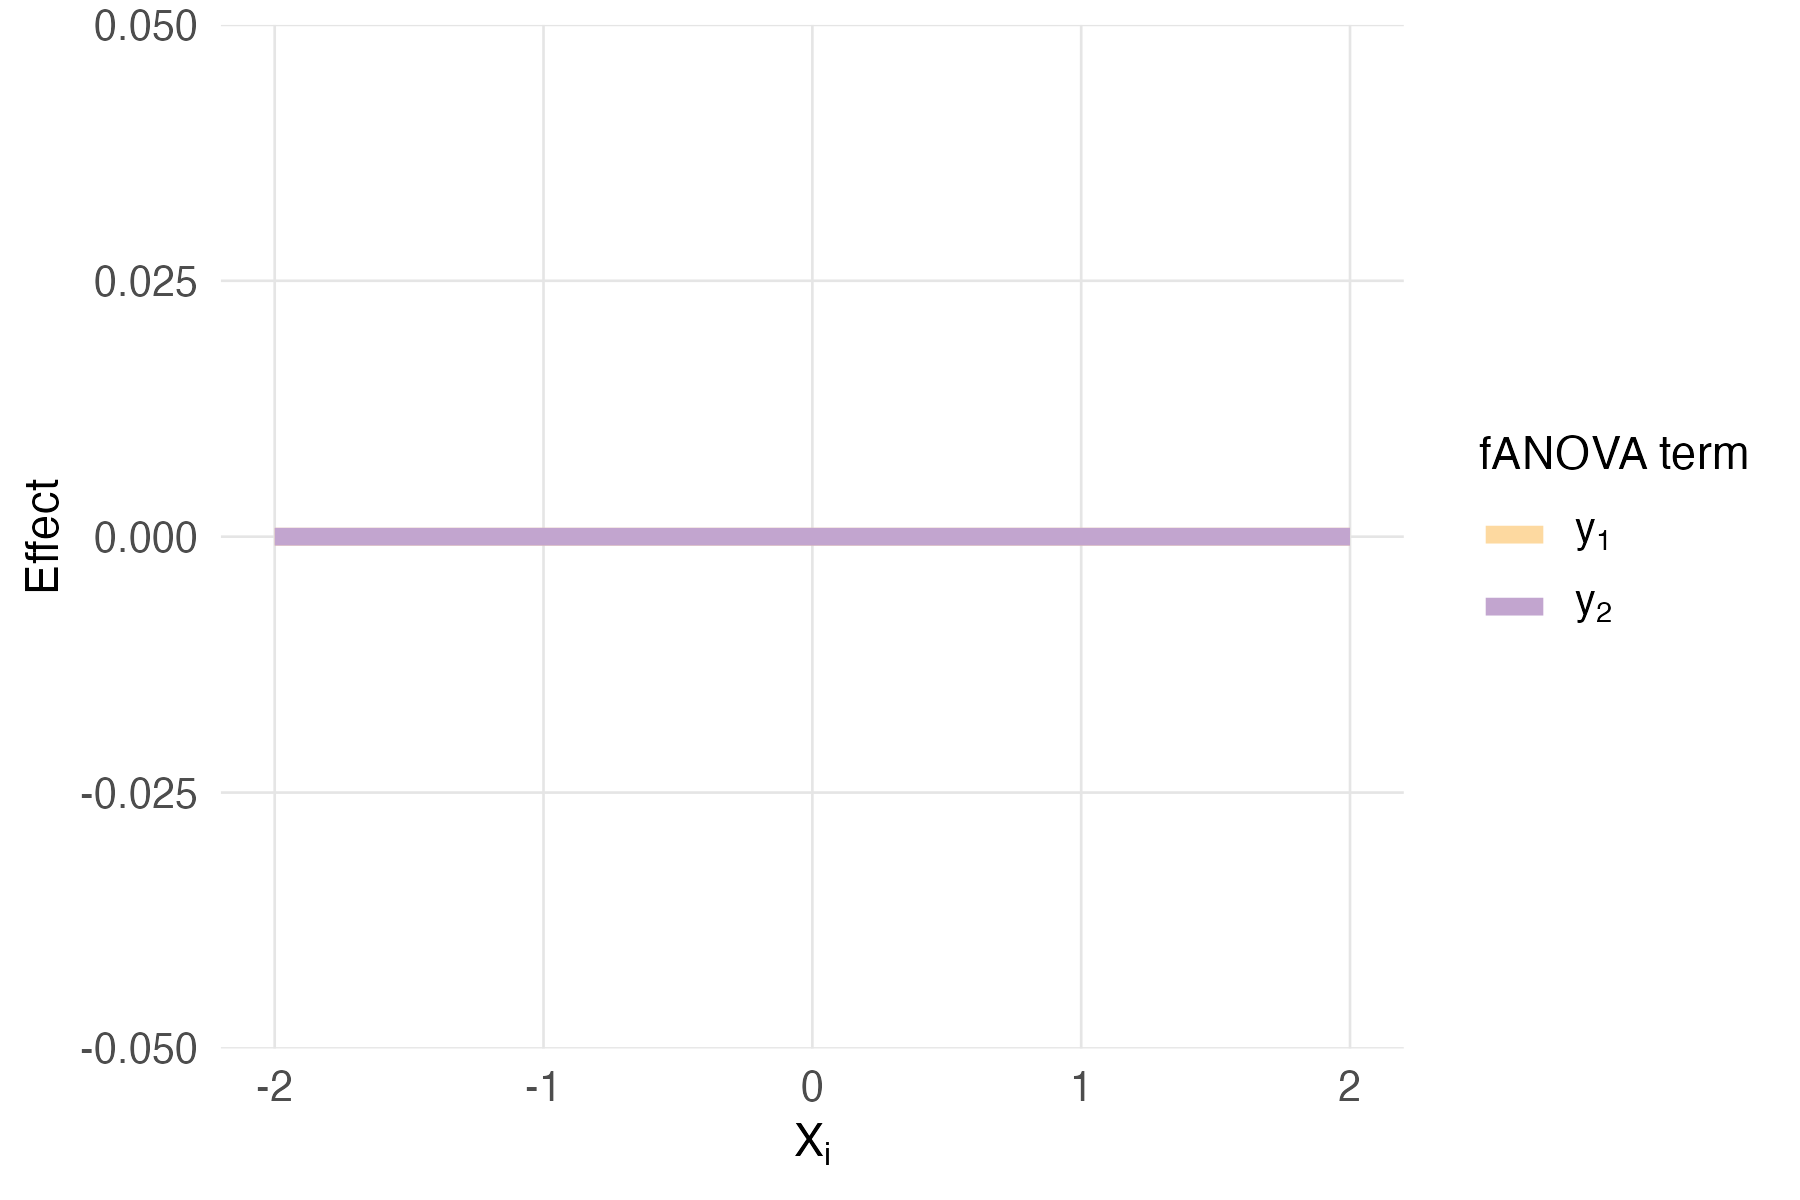
\includegraphics[width=\linewidth]{../images/experiment_section/interaction_a1p00_a2p00_a11p00_a22p00_a12p20_rhop00_main.png}
    \column{0.5\textwidth}
      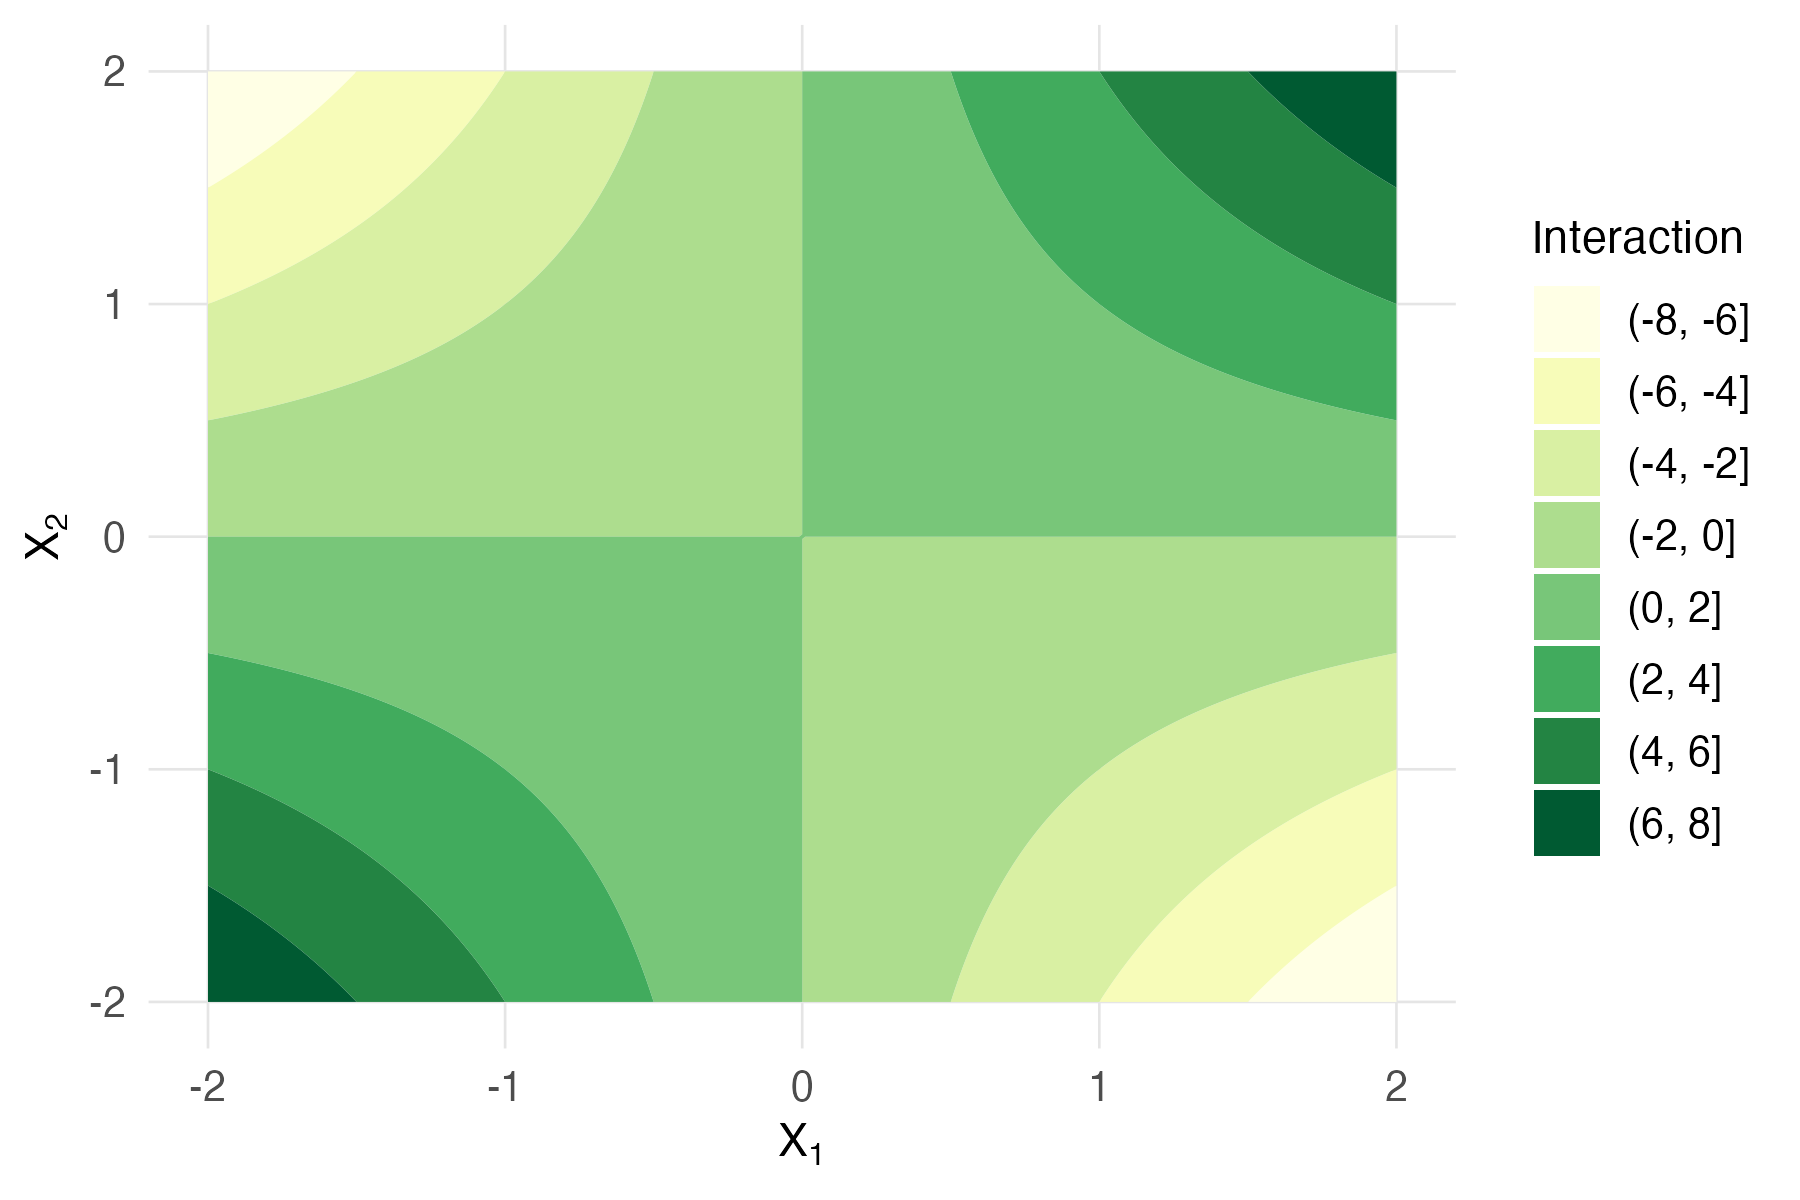
\includegraphics[width=\linewidth]{../images/experiment_section/interaction_a1p00_a2p00_a11p00_a22p00_a12p20_rhop00_interaction.png}
  \end{columns}
  
\end{frame}


\begin{frame}{Sobol Indices}
    Formula for classical Sobol' indices?
\end{frame}

\begin{frame}{Decomposition of linear functions}
  \begin{columns}
    \column{0.5\textwidth}
      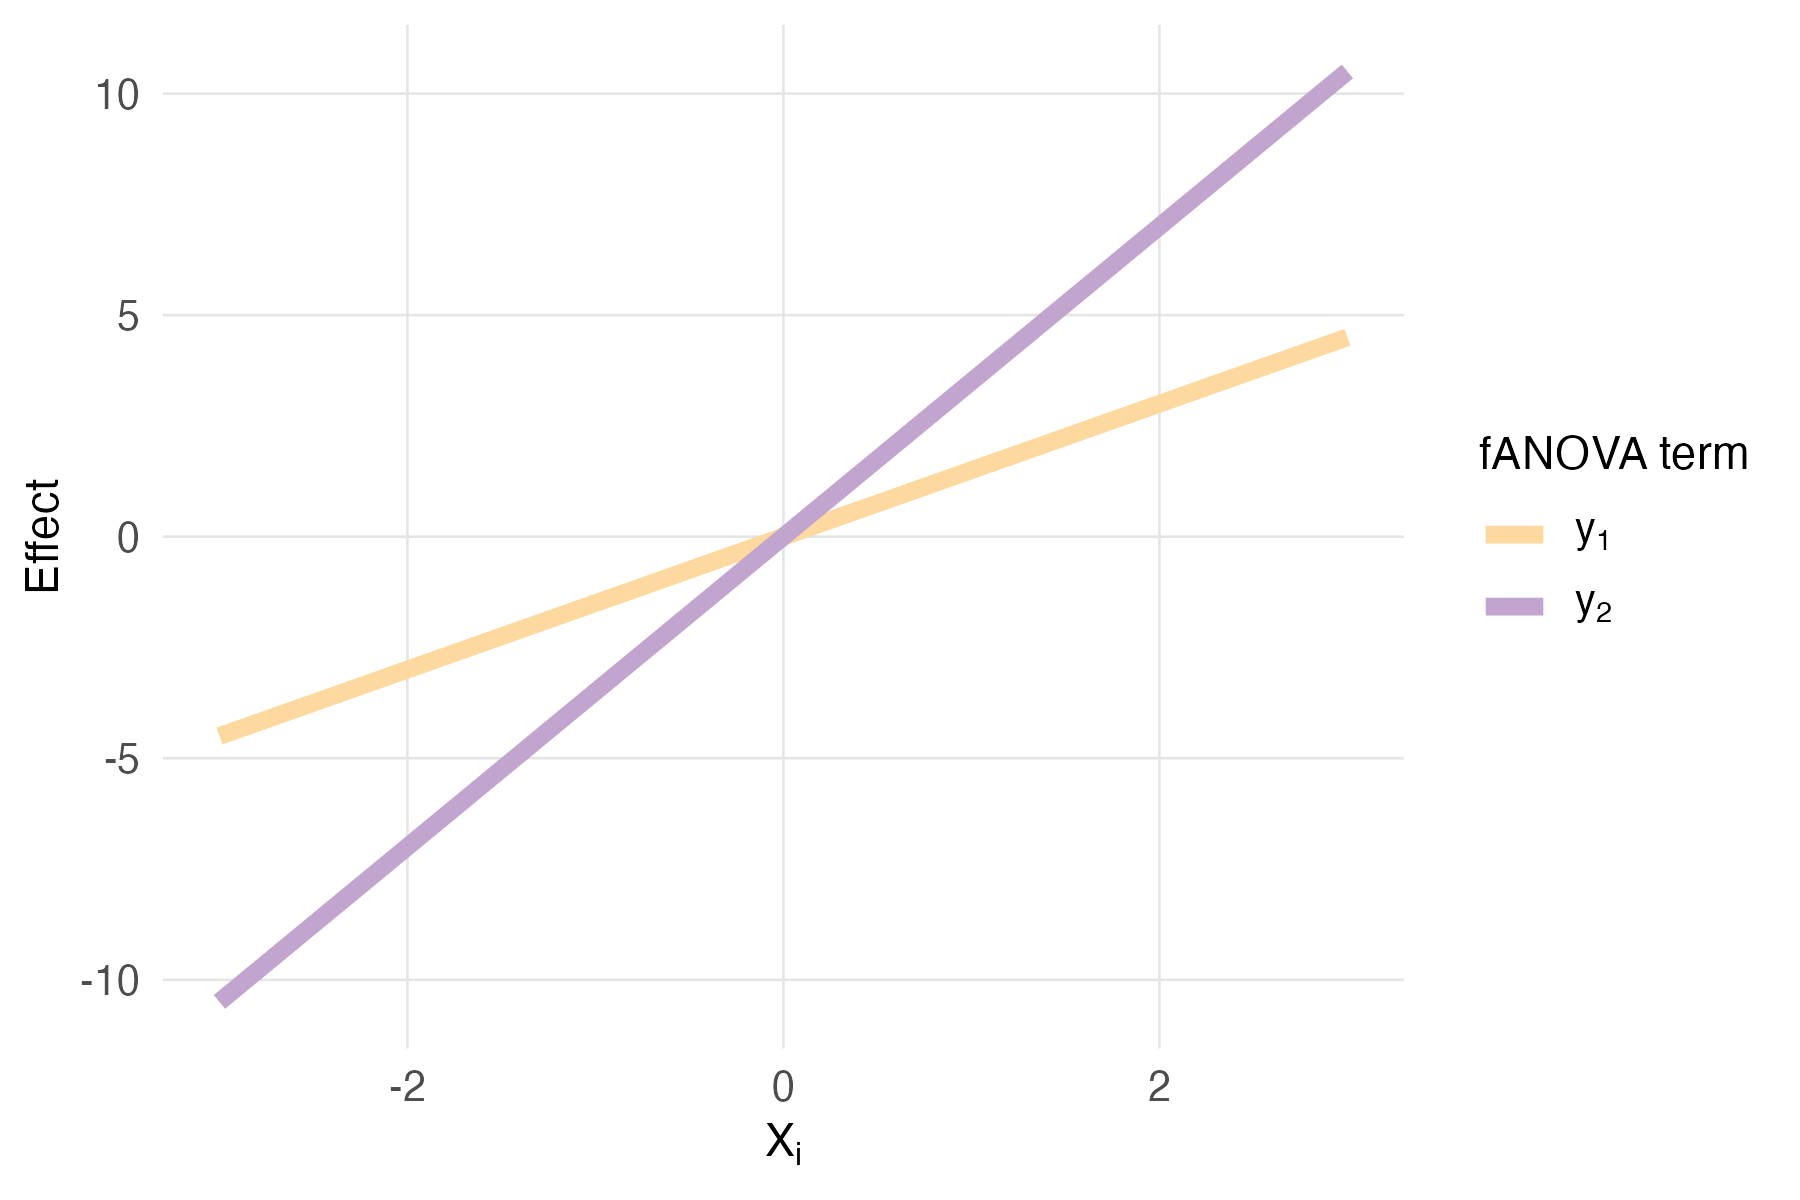
\includegraphics[width=\linewidth]{../images/experiment_section/linear_a1p15_a2p35_a11p00_a22p00_a12p00_rhop00_main.png}
      \captionof{figure}{$q(x_1, x_2) = 1.5 x_1 + 3.5 x_2$}
    \column{0.5\textwidth}
      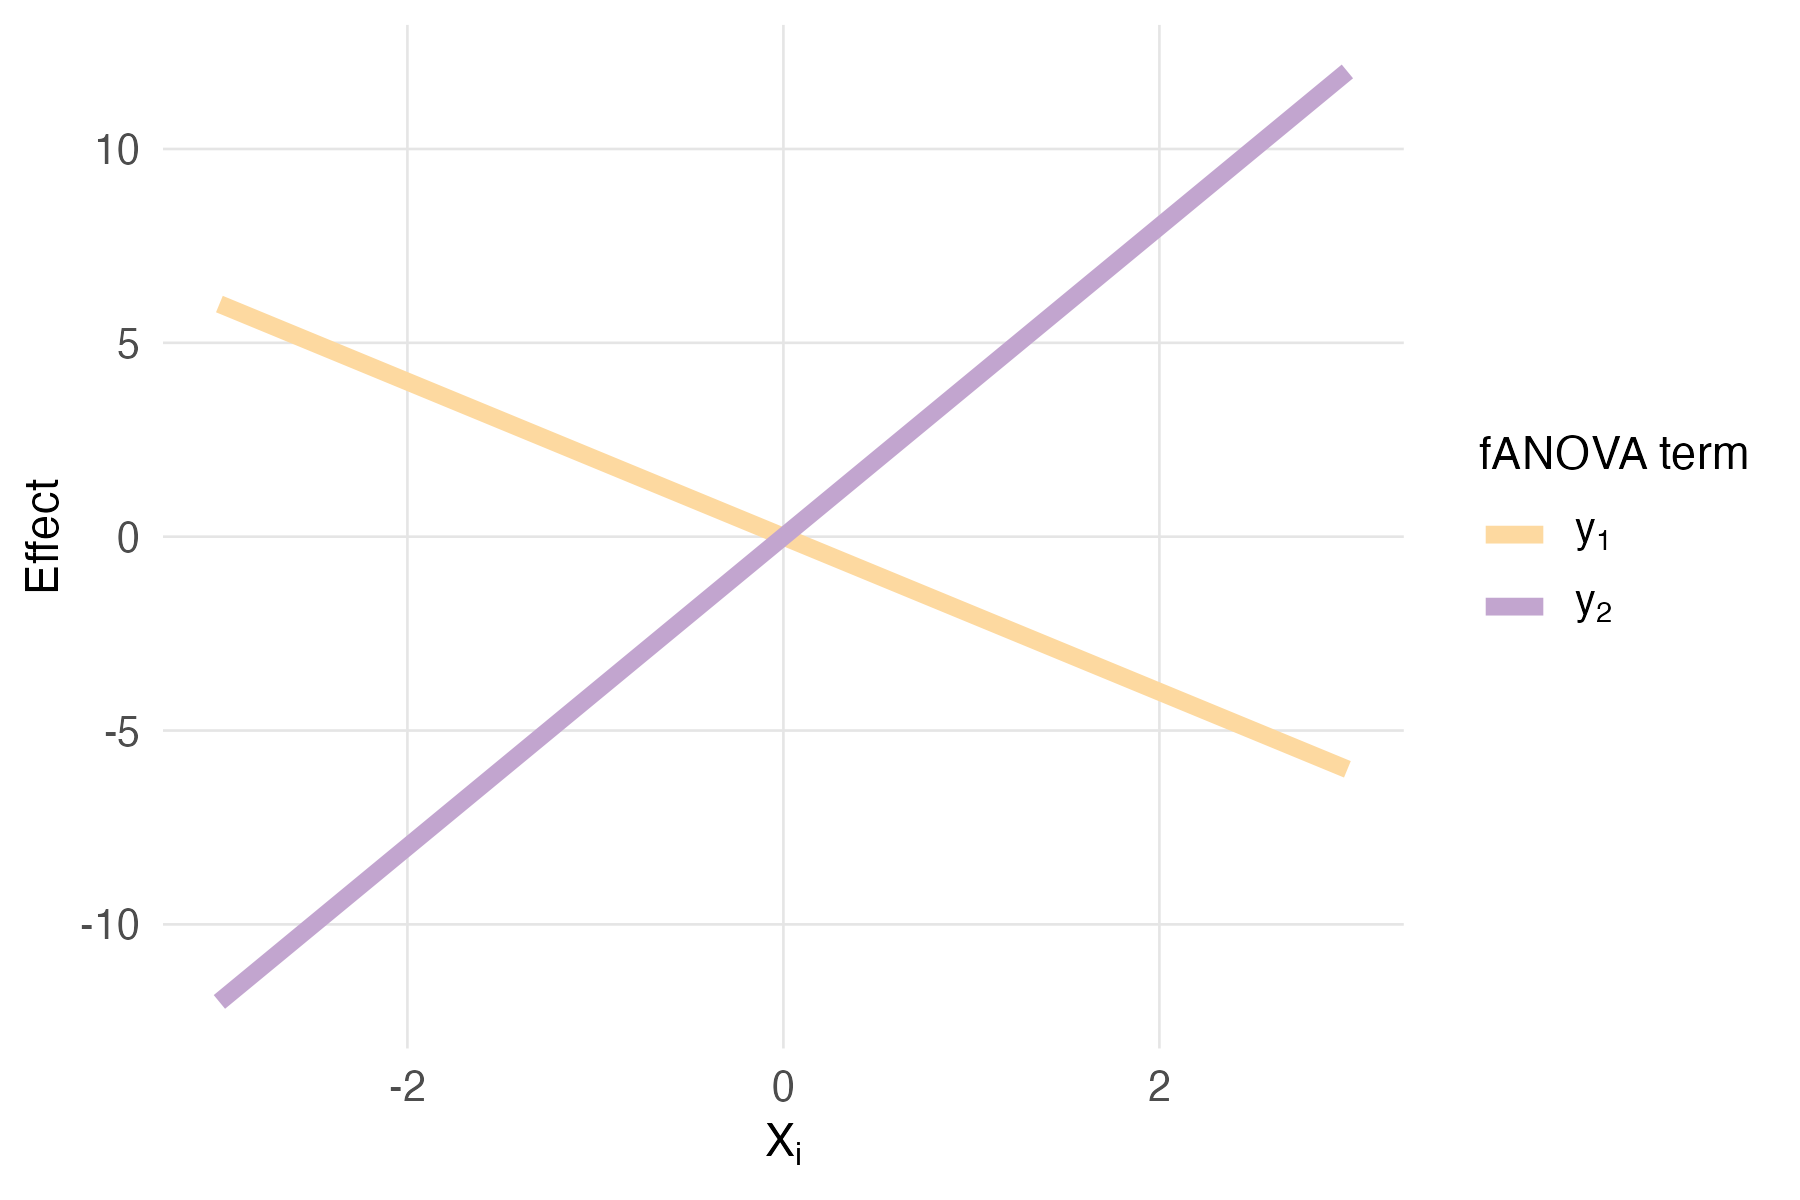
\includegraphics[width=\linewidth]{../images/experiment_section/linear_a1m20_a2p40_a11p00_a22p00_a12p00_rhop00_main.png}
      \captionof{figure}{$q(x_1, x_2) = -2 x_1 + 4 x_2$}
  \end{columns}
\end{frame}


\begin{frame}{Classical fANOVA Proofs}
    \begin{itemize}
        \item Zero mean property: factorized density, Fubinis Theorem, strong annihilating conditions
        \item Mutual orthogonality: factorized density, Fubinis Theorem, strong annihilating conditions
    \end{itemize}
\end{frame}

\begin{frame}{Generalized fANOVA Proofs}
    \begin{itemize}
        \item Zero mean property: separating $x$ into subvectors, marginal density, Fubinis Theorem, weak annihilating conditions
        \item Hierarchical orthogonality: set the scene, u is a proper subset of v $u \subsetneq v$, so there is an index in u which is not in v; divide $x_u$ into subvectors, marginal density, Fubini and weak annihilating conditions
        \item Weak annihilating becomes strong under independence: assume the weak ones, product density, factor out
        \item Three integration cases: distinguish between different relationships u and v, depending on the relationship the integral w.r.t. to marginal density simplifies
        \item Generalized fANOVA components by Rahman: first build constant term; for nonconstant terms use integration cases
        \item Integration constraint Hooker: show that hierarchical orthogonality is fulfilled if the conditions hold, show that it is not fulfilled if they do not hold; but why exactly these conditions a bit unclear
        \item Take a look at Sobols proof again
    \end{itemize}
\end{frame}

\begin{frame}{Relevant External Links}
    \begin{itemize}
        \item \url{https://docs.google.com/spreadsheets/d/1K5ECL6hDPDnHwM_k342xa29H-vHWzdk27PTgDHUwfFE/edit?usp=sharing} - Table with fANOVA-related literature
    \end{itemize}
\end{frame}